\documentclass{article}
\usepackage[margin=1in]{geometry}
\usepackage{graphicx}
\usepackage{float}
\usepackage{caption}
\usepackage{subcaption}
\usepackage[utf8]{inputenc}
\usepackage{amsfonts}
\usepackage{amsmath}
\usepackage{amssymb}

\usepackage{hyperref}
\usepackage{geometry}
\usepackage{dirtytalk}
\usepackage{parskip}
\usepackage{siunitx}
\usepackage{tikz}  
\usepackage{url}

\usepackage{booktabs}
\geometry{margin=1in}
\hypersetup{
    colorlinks=true,
    linkcolor=black,
    filecolor=black,      
    urlcolor=black,
    citecolor=blue,
    pdftitle={Overleaf Example},
    pdfpagemode=FullScreen,
}
\usepackage[titletoc]{appendix}

\title{\textbf{zkRisk}}
\author{\href{mailto:team@vest.xyz}{Vest Exchange}}
\date{November 2023}

\begin{document}

\maketitle

\tableofcontents

\section{Abstract}

We present a novel framework to unify the trading experience of digital assets and the money market such that the solvency of an exchange is guaranteed with high probability. This framework serves as the foundation for a trustless, composable financial ecosystem that enables the community to launch their own products while tapping into the deep liquidity of Vest. 

This paper outlines the construction of a perpetual futures exchange following this framework. Instead of a limit orderbook, traders trade against a liquidity pool composed of external liquidity providers (LPs) and an automated market maker (AMM) that prices shortfall risk using a coherent risk measure. 



\section{AMM}

\subsection{Motivation}

Prior attempts to develop trustless and scalable derivative exchanges through mechanisms like Constant Function Market Makers (CFMMs) and Limit Orderbooks (LOBs) have fallen short due to an inherent trade-off between risk management and efficient pricing.

On one hand, some exchanges guarantee solvency but result in less favorable pricing for traders, as observed in CFMMs where a basic formula dictates asset pricing. On the other hand, exchanges prioritizing better pricing often face higher insolvency risk, such as exchanges allowing trading directly on spot prices or LOBs due to the heterogeneity of independent market makers' risk profiles.

This poses a challenge: how can exchanges ensure liquidity without compromising pricing and risk?

\subsection{Overview}

Vest Exchange is a hybrid model that enforces a single coherent risk framework and responsively prices liquidity. It prices via. risk-indifference pricing, where the potential shortfall in the exchange's liability (long-short imbalance) is quantified using a coherent risk measure. The control variables are premia and funding, which directly reduce risk and incentivize the reduction of liability.

\subsection{Coherent Risk Measure}\label{risk}
Consider $n$ markets, where the underlying assets follow price process $S_t = \begin{pmatrix} S^{(1)}_t \\ \vdots \\ S^{(n)}_t\end{pmatrix} \in \mathbb{R}^n_{++}$ adapted on a filtered probability space $(\Omega, \mathcal{F}, \{\mathcal{F}_t\}_{0\leq t \leq \tau}, \mathbb{P})$.

We define the exchanges's liability at time $t$ as a function of $S_t$, parameterized by the state of the exchange $\theta = (\mathbf{q}, C, P, L)$

\begin{equation}
    X_t(\theta) 
    := f(S_t;\theta)= \mathbf{q}^TS_t-(C+P+L)
\end{equation}

where $\mathbf{q} \in \mathbb{R}^n$ is a vector of long-short imbalances ($ q_i > 0$ implies that the $i$th market is long-heavy, hence AMM is net short), $C = \mathbf{q}^T\overline{\mathbf{s}} \in \mathbb{R}$ is the summation of entry notional sizes (signed) of all open positions, $P \in \mathbb{R}_+$ is capital owned by the AMM, and $L \in \mathbb{R}_+$ is capital provided by LPs (see Section \ref{lp}). In other words, $X_t$ represents the net payout to traders if all outstanding positions were to be closed at prices $S_t$. 

We use a monetary risk measure, a mapping from a set of random variables to the real numbers, to calculate the amount of capital needed to cover the potential shortfall with high probability. In particular, we use an extension of a coherent risk measure called Entropic Value-at-Risk (EVaR) \cite{ahmadi2012entropic}.

EVaR is the tightest upper bound to Value-at-Risk (VaR) and Conditional Value-at-Risk (CVaR) derived from the Chernoff bound $P(X\geq a) \leq e^{-za}M_X(z)=\alpha$, solving for $a$:
\begin{equation}
    \text{EVaR}_{1-\alpha}(X) = \inf_{z > 0} \{ z^{-1} \ln \frac{M_X(z)}{\alpha} \}
\end{equation}

for a confidence level $1-\alpha$. 

Using EVaR, zkRisk charges premia and funding to guarantee solvency with respect to rolling windows $[t,t+\tau]$ by ensuring the following invariant holds with high probability at $t$:

\begin{equation}\label{eq:solvency}
    X_{t+\tau} < 0.
\end{equation}

We define our risk measure as
\begin{gather}\label{eq:risk}
    \rho(X_{t+\tau}|\mathcal{F}_t) := \text{EVaR}_{1-\alpha}(X_{t+\tau}^+ - P_t|\mathcal{F}_t) \\ 
    P_t = \sum_{s=t-\tau}^t \pi^\rho_s + f^\rho_s 
\end{gather}

where $\pi^\rho$ and $f^\rho$ are premium and funding collected by AMM respectively (\ref{premia} and \ref{funding}). We take $(\cdot)^+ = \max(0, \cdot)$ to ignore upside (negative shortfall). This particular construction is coherent (see Appendix \ref{app1}).

\subsection{Premia}\label{premia}

For a new trade $\mathbf{q}_t \in \mathbb{R}^n$, zkRisk charges premium or provides rebate such that the risk before and after accepting the trade remains invariant. In particular, we define the premium as
\begin{equation}\label{risk-indiff}
    \pi^\rho_t := (\rho(X_{t+\tau}(\theta') | \mathcal{F}_t) -
    \rho(X_{t+\tau}(\theta)|\mathcal{F}_t))^+
\end{equation}
where $\theta = (\mathbf{q}, C, P, L)$ and $\theta' = (\mathbf{q}+\mathbf{q}_t, C+\mathbf{q}_t^TS_t, P, L)$ represent states before and after accepting the trade. At $t+\tau$, AMM-owned capital $P$ is incremented by $\pi_t^\rho$.

\subsection{Funding}\label{funding}

While premia charges for marginal change in risk from the change in liability, zkRisk needs to collect funding from open positions to cover the market risk.

Given our risk measure is 1-positive homogenous (see Appendix \ref{app1}), we use a risk attribution mechanism called Euler allocation to define per-market funding rate. Let $X_{t}^{(i)}$ be the liability arising from $i$th market. We calculate the amount of funding assigned to the $i$th market as

\begin{equation}
    \rho_{Euler}(X_{t+\tau}^{(i)}|\mathcal{F}_{t}):= \frac{\partial\rho(\sum_{i=1}^n u_i X_{t+\tau}^{(i)} |\mathcal{F}_t)}{\partial u_i}|_{(1,\dots,1)}.
\end{equation}

This represents the marginal risk added by long-short imbalance in the $i$th market. We now define instantaneous funding charged across all open positions as

\begin{equation}\label{risk-indiff-funding}
f^\rho_t(X^{(i)}_{t+\tau}|\mathcal{F}_t) := \frac{\partial \rho_{Euler}(X_{t+\tau}^{(i)}|\mathcal{F}_t)}{\partial \tau} |_{\tau}
\end{equation}

which corresponds to the marginal change in risk with respect to time. 

Now, for each trader $j \in I_i$ with position size $q_{i_j} \in \mathbb{R}$ where $\sum_{j\in I_i}q_{i_j}=q_{i}$, they are responsible for covering 

\begin{equation}
    f^\rho_t(X^{(i)}_{t+\tau}|\mathcal{F}_t)\frac{q_{i_j}}{q_{i}}.
\end{equation} 

$f^\rho_t(X^{(i)}_{t+\tau}|\mathcal{F}_t)\frac{q_{i_j}}{q_{i}} > 0$ means trader $j$ pays the funding and they receive it otherwise.

Similar to premium, $P$ will be incremented at time $t+\tau$ with funding charged at time $t$. Derivation of the exact formulas are deferred to Appendix \ref{app2}.

\section{LPs}\label{lp}
\subsection{Overview}
LPs receive rewards for underwriting potential shortfall by committing capital $L$. 

Suppose LPs commit aggregate capital $L$. Given the exchange's state $\theta = (\mathbf{q}, C, P, L)$, we represent the inventory $\mathbf{q}$ as a single virtual asset whose price follows a univariate normal distribution $S^v_{t} \sim \mathcal{N}(\mathbf{q}^T \boldsymbol{\mu}_{t}, \mathbf{q}^T \mathbf{\Sigma}_{t} \mathbf{q})$, where $S_t \sim \mathcal{N}(\boldsymbol{\mu}_{t}, \boldsymbol{\Sigma}_{t})$. With respect to such contract, the AMM has average entry price $\bar{s}^v = C$ and default price $d^v = \bar{s}^v + P + L$.

\begin{figure}
\begin{center}


\tikzset{every picture/.style={line width=0.75pt}} %set default line width to 0.75pt        

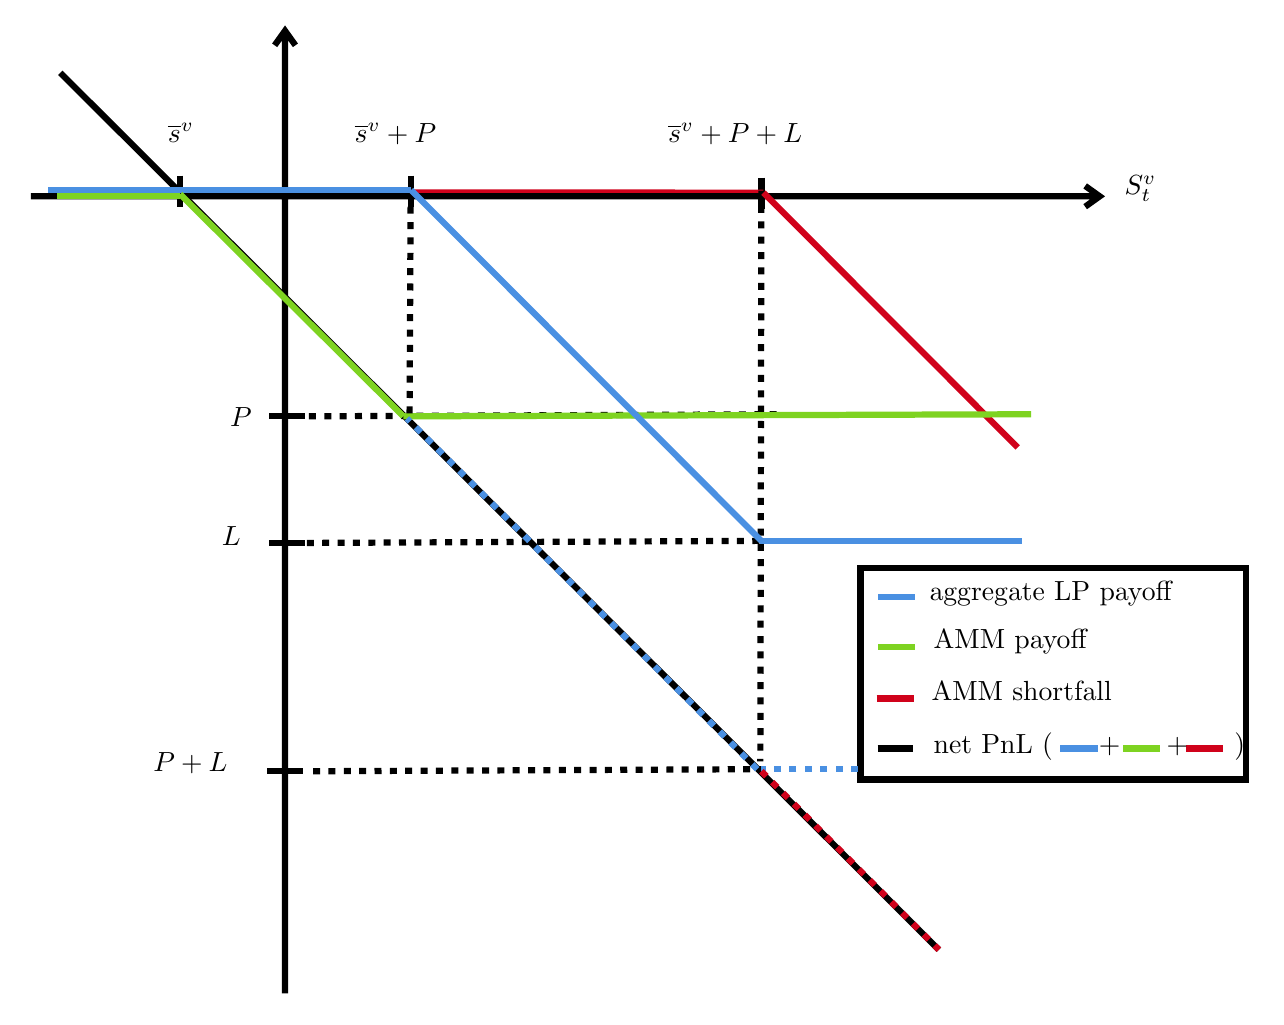
\begin{tikzpicture}[x=0.75pt,y=0.75pt,yscale=-1,xscale=1]
%uncomment if require: \path (0,541); %set diagram left start at 0, and has height of 541

%Straight Lines [id:da31599197893864994] 
\draw [line width=2.25]    (380.25,104.75) -- (380.25,119.75) ;
%Straight Lines [id:da5755907536064695] 
\draw [color={rgb, 255:red, 208; green, 2; blue, 27 }  ,draw opacity=1 ][line width=2.25]    (68.25,111.75) -- (381.25,112) ;
%Straight Lines [id:da40964072115610617] 
\draw [line width=2.25]  [dash pattern={on 2.53pt off 3.02pt}]  (380.25,111) -- (379.75,386) ;
%Shape: Axis 2D [id:dp414111847638135] 
\draw [line width=2.25]  (28.25,113.75) -- (543.25,113.75)(150.75,34) -- (150.75,497.75) (536.25,108.75) -- (543.25,113.75) -- (536.25,118.75) (145.75,41) -- (150.75,34) -- (155.75,41)  ;
%Straight Lines [id:da6267893935238507] 
\draw [line width=2.25]    (100.25,103.75) -- (100.25,118.75) ;
%Straight Lines [id:da9686890438584196] 
\draw [line width=2.25]    (211.25,103.75) -- (211.25,118.75) ;
%Straight Lines [id:da7391904760440071] 
\draw [line width=2.25]    (42.5,54.25) -- (465.75,476.75) ;
%Straight Lines [id:da5677235487377026] 
\draw [color={rgb, 255:red, 74; green, 144; blue, 226 }  ,draw opacity=1 ][line width=2.25]    (505.75,279.75) -- (379.75,279.75) ;
%Straight Lines [id:da9306805248897732] 
\draw [color={rgb, 255:red, 74; green, 144; blue, 226 }  ,draw opacity=1 ][line width=2.25]    (211.5,110.75) -- (36.75,110.75) ;
%Shape: Rectangle [id:dp8104244130615202] 
\draw  [line width=2.25]  (428,292.75) -- (613.75,292.75) -- (613.75,394.75) -- (428,394.75) -- cycle ;
%Straight Lines [id:da7317866741344016] 
\draw [color={rgb, 255:red, 74; green, 144; blue, 226 }  ,draw opacity=1 ][line width=2.25]    (454.25,306.75) -- (436.25,306.75) ;
%Straight Lines [id:da6594018061849531] 
\draw [line width=2.25]    (142.25,390.75) -- (159.25,390.75) ;
%Straight Lines [id:da9587445248445144] 
\draw [line width=2.25]    (143.25,280.75) -- (160.25,280.75) ;
%Straight Lines [id:da2622020295016816] 
\draw [line width=2.25]  [dash pattern={on 2.53pt off 3.02pt}]  (161.25,280.75) -- (379.75,279.75) ;
%Straight Lines [id:da05623222756798141] 
\draw [color={rgb, 255:red, 208; green, 2; blue, 27 }  ,draw opacity=1 ][line width=2.25]    (435.75,355.75) -- (453.75,355.75) ;
%Straight Lines [id:da45174941449663786] 
\draw [color={rgb, 255:red, 208; green, 2; blue, 27 }  ,draw opacity=1 ][line width=2.25]    (381.25,112) -- (503.75,234.75) ;
%Straight Lines [id:da9755211019000269] 
\draw [line width=2.25]    (143.25,219.75) -- (160.25,219.75) ;
%Straight Lines [id:da06453399583039221] 
\draw [line width=2.25]    (436.25,379.75) -- (453.25,379.75) ;
%Straight Lines [id:da9394063236161404] 
\draw [line width=2.25]  [dash pattern={on 2.53pt off 3.02pt}]  (162.25,219.75) -- (389.25,218.75) ;
%Straight Lines [id:da67892975305957] 
\draw [color={rgb, 255:red, 126; green, 211; blue, 33 }  ,draw opacity=1 ][line width=2.25]    (100.25,112.75) -- (207.75,219.75) ;
%Straight Lines [id:da15467716636967233] 
\draw [color={rgb, 255:red, 126; green, 211; blue, 33 }  ,draw opacity=1 ][line width=2.25]    (510.25,218.75) -- (207.75,219.75) ;
%Straight Lines [id:da565173472771882] 
\draw [color={rgb, 255:red, 126; green, 211; blue, 33 }  ,draw opacity=1 ][line width=2.25]    (454.25,330.75) -- (436.25,330.75) ;
%Straight Lines [id:da7777261369150089] 
\draw [color={rgb, 255:red, 126; green, 211; blue, 33 }  ,draw opacity=1 ][line width=2.25]    (572.25,379.75) -- (554.25,379.75) ;
%Straight Lines [id:da16355037680968265] 
\draw [color={rgb, 255:red, 74; green, 144; blue, 226 }  ,draw opacity=1 ][line width=2.25]    (542.25,379.75) -- (524.25,379.75) ;
%Straight Lines [id:da12556440160685256] 
\draw [color={rgb, 255:red, 208; green, 2; blue, 27 }  ,draw opacity=1 ][line width=2.25]    (584.75,379.75) -- (602.75,379.75) ;
%Straight Lines [id:da4399081729533382] 
\draw [line width=2.25]  [dash pattern={on 2.53pt off 3.02pt}]  (164.25,390.75) -- (380.25,389.75) ;
%Straight Lines [id:da8111809512706335] 
\draw [line width=2.25]  [dash pattern={on 2.53pt off 3.02pt}]  (211.25,118.75) -- (210.75,219.75) ;
%Straight Lines [id:da31921719668647186] 
\draw [color={rgb, 255:red, 126; green, 211; blue, 33 }  ,draw opacity=1 ][line width=2.25]    (100.25,113.75) -- (40.75,113.75) ;
%Straight Lines [id:da03694710779533339] 
\draw [color={rgb, 255:red, 74; green, 144; blue, 226 }  ,draw opacity=1 ][line width=2.25]    (380.25,279.75) -- (211.5,110.75) ;
%Straight Lines [id:da8797126299874389] 
\draw [color={rgb, 255:red, 74; green, 144; blue, 226 }  ,draw opacity=1 ][line width=2.25]  [dash pattern={on 2.53pt off 3.02pt}]  (378.25,389.75) -- (209.5,220.75) ;
%Straight Lines [id:da6303640240129449] 
\draw [color={rgb, 255:red, 74; green, 144; blue, 226 }  ,draw opacity=1 ][line width=2.25]  [dash pattern={on 2.53pt off 3.02pt}]  (426.75,389.75) -- (380.25,389.75) ;
%Straight Lines [id:da6779929874717828] 
\draw [color={rgb, 255:red, 208; green, 2; blue, 27 }  ,draw opacity=1 ][line width=2.25]  [dash pattern={on 2.53pt off 3.02pt}]  (380.25,390.75) -- (465.75,476.75) ;

% Text Node
\draw (93,77.4) node [anchor=north west][inner sep=0.75pt]    {$\overline{s}^{v}$};
% Text Node
\draw (183,77.4) node [anchor=north west][inner sep=0.75pt]    {$\overline{s}^{v} +P$};
% Text Node
\draw (334,77.4) node [anchor=north west][inner sep=0.75pt]    {$\overline{s}^{v} +P+L$};
% Text Node
\draw (460,298) node [anchor=north west][inner sep=0.75pt]   [align=left] {aggregate LP payoff};
% Text Node
\draw (86,380.4) node [anchor=north west][inner sep=0.75pt]    {$P+L$};
% Text Node
\draw (119,271.4) node [anchor=north west][inner sep=0.75pt]    {$L$};
% Text Node
\draw (461,346) node [anchor=north west][inner sep=0.75pt]   [align=left] {AMM shortfall};
% Text Node
\draw (123,214.4) node [anchor=north west][inner sep=0.75pt]    {$P$};
% Text Node
\draw (462,371) node [anchor=north west][inner sep=0.75pt]   [align=left] {net PnL ( \ \ \ \ + \ \ \ \ + \ \ \ \ ) };
% Text Node
\draw (462,321) node [anchor=north west][inner sep=0.75pt]   [align=left] {AMM payoff};
% Text Node
\draw (554,102.4) node [anchor=north west][inner sep=0.75pt]    {$S_{t}^{v}$};

\end{tikzpicture}
\end{center}
\caption{Exchange payoff graph}
\label{fig:payoff}
\end{figure}

From Figure \ref{fig:payoff}, observe that LPs take on the entire liability after the AMM has run out of capital $P$ by taking on a bounded payoff $Y_t$ where

\begin{equation}
Y_t := -(S^v_t - (\bar{s}^v + P))^+ + (S^v_t - (\bar{s}^v+P+L))^+ 
\end{equation}

which is equivalent to the payoff of selling a call spread on the virtual asset. 

\subsection{Premia}

We can view the total exchange risk as being composed of an unhedgeable component taken on by the AMM and a hedgeable component taken on by the LPs.

Thus, we define the premium given to LPs of a new trade $\mathbf{q}_t$ as

\begin{equation}
    \pi_t^L := (C_{K_1(\theta'), K_2(\theta')}(t,t+\tau) -  C_{K_1(\theta), K_2(\theta)}(t,t+\tau))^+
\end{equation}

where $C_{K_1, K_2}(t, T)$ is the price of a call spread with strikes $K_1 < K_2$ at $t$ expiring at $T$, $K_1(\theta) = C + P$ and $K_2(\theta) = C+P+L$. 

\subsection{Funding}

Similar to (\ref{risk-indiff-funding}), LPs will collect funding from traders. We define total instantaneous funding $f^L_t$ charged across all open positions per unit time as

\begin{equation}
    f^L_t := \frac{\partial C_{K_1,K_2}(t,t+\tau)}{\partial \tau} |_{\tau}
\end{equation}

(12) is distributed among all markets using Euler allocation.

\subsection{Withdrawal}
An LP may declare to withdraw capital $l$ at $t$ by keeping it locked until $t+\tau$. Otherwise, one may force withdraw without waiting, say at $s < t+\tau$, 
with a risk-indifference fee 

\begin{equation}
    \rho(X_{t+\tau}(\theta')|\mathcal{F}_{s}) -\rho(X_{t+\tau}(\theta)|\mathcal{F}_{s})
\end{equation}

where $\theta = (\mathbf{q}, C, P, L)$ and $\theta' = (\mathbf{q}, C, P, L - l)$. This ensures that the force withdrawal of capital does not impact the risk level of the AMM.

\section{Risk Engine}

\subsection{Volatility Forecast}\label{vol}

First, we cluster assets into groups with cointegrated time series of log returns. Then, we forecast the covariance within each group. Let $\{\mathbf{r}_t\} \in \mathbb{R}^n$ be a vector stochastic process of standardized log returns. We assume the following model:

\begin{equation}
\mathbf{r}_t \mid \mathcal{F}_{s} \sim \mathcal{N}(0, \mathbf{\Sigma}_t)
\end{equation}

for $s \leq t$ where $\mathcal{F}_{s}$ is the information up to time $s$ and $\mathbf{\Sigma}_t$ is the covariance matrix that we wish to forecast.

We assume that there exist unobservable factors $\mathbf{f}_t$ that are conditionally heteroscedastic and generate the log returns $\mathbf{r}_t$ for a set of assets. That is, 
\begin{equation}
    \mathbf{r}_t = \mathbf{Z} \mathbf{f}_t
\end{equation}
where $\mathbf{Z}$ is a time-invariant linear map. We argue that such an assumption is justified in the speculative context of cryptocurrencies where price movements are often highly correlated. 

We use Generalized Orthogonal-GARCH (GO-GARCH) \cite{van2002go} because it outperforms other models such as univariate GARCH and DCC-GARCH in our backtests \cite{vest2023vol}. GO-GARCH allows $\mathbf{Z}$ to be (left) invertible and parameterizes $\mathbf{Z}$ with singular value decomposition:

\begin{equation}
    \mathbf{\Sigma}_t = \mathbf{Z} \mathbf{D}_t \mathbf{Z}^T,\ \mathbf{Z} = \mathbf{Q} \boldsymbol{\Lambda} \mathbf{U}^T
\end{equation}

where $\mathbf{D}_t = diag(\sigma^2_{f_{t,1}}, \ldots, \sigma^2_{f_{t, n}})$ is a diagonal matrix of the conditional variances of each factor modeled by univariate GARCH. $\mathbf{Z} = \mathbf{Q}\boldsymbol{\Lambda}\mathbf{U}^T$ is the $n \times n$ mixing matrix outputted by Independent Component Analysis \cite{ghalanos2019rmgarch}. 

% Future work for volatility forecasting includes applying a hidden Markov model to consider transitions between high volatility and low volatility regimes to model the volatility process for each of the factors \cite{li2019improve} or even allowing the factor loading matrix $\mathbf{Z}$ to be state dependent \cite{saidane2009optimal}.

\subsection{Liquidations} \label{liq}
If the portfolio value for a trader becomes less than the maintenance margin requirement, open positions will be closed partially or fully in order to bring the account value back to a healthy level (above the initial margin requirement). 

Currently the liquidator runs an \href{https://research.vest.xyz/t/optimal-liquidations-via-convex-optimization/201}{optimal liquidation solver} in order to prevent excessive liquidations for traders as well as to minimize the negative externalities such as liquidation cascades. 

In particular, liquidation of a portfolio $\mathbf{q}_j$ is formalized as a convex optimization problem: 
\begin{align} 
    \underset{\mathbf{w}}{\text{minimize}} \quad & \sum_{i=1}^nw_iq_j^{(i)}S_{t}^{(i)} \\ \text{subject to} \quad &\mathbf{0} \preceq \mathbf{w} \preceq \mathbf{1} \\ 
    & (r + \epsilon)\sum_{i=1}^n(1-w_i)|q_j^{(i)}|S_{t}^{(i)}  \leq c - \pi + \sum_{i=1}^n(S_{t}^{(i)}-s_{entry}^{(i)})q_j^{(i)} \\
    &\pi = (\rho(X_{t+\tau}(\theta')|\mathcal{F}_t)-\rho(X_{t+\tau}(\theta)|\mathcal{F}_t))^+\\
    &\theta = (\mathbf{q}, C, P, L) \\
    &\theta' = (\mathbf{q}-(\mathbf{1}-\mathbf{w})\mathbf{q}_j, C-(\mathbf{1}-\mathbf{w})\mathbf{q}_j^TS_t, P, L)
\end{align}

where $\mathbf{w}$ is the optimal liquidation weight that we solve for, $S_{entry}^{(i)}$ and $\mathbf{q}_j^{(i)}$ are entry price and signed position size for position $i$, $c$ is the collateral, and $\pi$ is the liquidation fee. Note that the liquidation fee (23) is convex in $\mathbf{w}$, as it is determined by risk measure $\rho$ which is convex in $\mathbf{w}$, and the second term $\rho(X_{t+\tau}(\theta)|\mathcal{F}_t)$ is a constant.

\section{Verifying Off-Chain Computation}

Due to the computational complexity of the pricing mechanism and risk engine, we offload computations off-chain and produce proof of correctness that can be verified on-chain. 

\subsection{Proof of Computation}

Using zkSNARKs, we prove correctness of the pricing by first proving that the forecasted covariance matrix is outputted by the declared model (\ref{vol}) given a vector of market prices. Then, given the forecasted covariance matrix, we prove that the pricing of premia (\ref{risk-indiff}) and funding (\ref{risk-indiff-funding}) is computed according to their respective risk-indifference formulas. The resulting risk measure is also be posted on chain.

\subsection{Proof of Optimality}

Liquidations (\ref{liq}) are formulated as convex optimization problems. By exploiting strong duality, we prove that a given solution is optimal with zkSNARKs by proving that it is feasible for both the primal and dual problems and that the duality gap is zero (up to some precision errors) \cite{angel2022efficient}. We then leverage state-of-the-art solvers off-chain. This also implies we can decentralize the running of these solvers and reward solutions based on speed.

\bibliographystyle{alpha}
\bibliography{bibliography.bib}

\begin{appendices}
\section{Risk Measure Properties} \label{app1}
Here, we show our risk measure is coherent, assuming the underlying prices are normally distributed. 

\begin{itemize}
    \item[(P1)] Normalized: $\rho(0)=0$
    \item[(P2)] Monotone: if $X(\theta_1) \leq X(\theta_2)$ almost surely (which is the case if and only if $\mathbf{q}_1 = \mathbf{q_2}$ and $\mathbf{q}_1^T\mathbf{\overline{s}}_1+P+L\leq \mathbf{q}_2^T\mathbf{\overline{s}}_2+P_2+L$), then $\rho(X(\theta_1)) \geq \rho(X(\theta_2))$. 
    \item[(P3)] Convex: $\rho(\lambda X(\theta_1) + (1-\lambda) X(\theta_2)) \leq \lambda\rho(X(\theta_1))+(1-\lambda)\rho(X(\theta_2))$
    \item[(P4)] (1-)Positive Homogenoeus: $\rho(\lambda X) = \lambda \rho(X)$ for $\lambda \geq 0$
\end{itemize}

Verifying (P1) and (P2) is straight forward. One key idea in showing (P3) and (P4) is that EVaR with confidence level $1-\alpha$ is equivalent to expected value under equivalent probability measure obtained using Esscher transform with parameter $h$. Such $h$ is uniquely determined by $\alpha$ \cite{chengli2012coherent}. In the case of Normal random variable, which is the assumption we work under, Esscher transform of the distribution is also Normal, with the same variance $\sigma$ and mean shifted by $h\sigma^2$. From here on, we denote by $E_h(f_X)$ the Esscher transform of probability density function $f_X$.

For (P4), we have 
\begin{align*}
    \rho(\lambda X) 
    &= EVaR_{1-\alpha}[\lambda(X^+-P)]\\
    &= E_{E_h(f_{\lambda \mathbf{q}^TS})}[\lambda (X^+-P)] \\
    &=\lambda(\mu-(\mathbf{q}^T\overline{\mathbf{s}}+P+L))\Phi(\frac{\lambda(\mu-(\mathbf{q}^T\overline{\mathbf{s}}+P+L))}{\lambda\sigma})+\lambda\sigma\phi(\frac{\lambda(\mu-(\mathbf{q}^T\overline{\mathbf{s}}+P+L))}{\lambda\sigma}) -\lambda P\\
    &= \lambda E_{E_h(f_{\mathbf{q}^TS})}[X^+-P]\\
    &= \lambda EVaR_{q-\alpha}[X^+-P]\\
    &= \lambda\rho(X)
\end{align*}

where $\mathbf{q}^TS \sim \mathcal{N}(\mu, \sigma)$.

For (P3), we have
\begin{align*}
&\ \lambda \rho(X(\theta_1)) + (1-\lambda)\rho(X(\theta_2)) \\
=&\  E_{E_h(f_{\lambda\mathbf{q_1}^TS})}[\lambda X(\theta_1)^+]+E_{E_h(f_{\lambda\mathbf{q_2}^TS})}[\lambda X(\theta_2)^+]\\
= &\ E_{f_S}[\lambda (\mathbf{q}_1^TS-(C_1-\sqrt{-2\ln\alpha\mathbf{q}_1^T\boldsymbol{\Sigma}\mathbf{q}_1}))^+] 
+ E_{f_S}[(1-\lambda) (\mathbf{q}_2^TS-(C_2-\sqrt{-2\ln\alpha\mathbf{q}_2^T\boldsymbol{\Sigma}\mathbf{q}_2}))^+]  \\
&\ \quad(C_i := \mathbf{q}_i^T\mathbf{\overline{s}}_i+P_i+L_i)\\
\geq &\ E_{f_S}[((\lambda\mathbf{q}_1+(1-\lambda)\mathbf{q}_2)^TS + \sqrt{ -2\ln\alpha}(\lambda \sqrt{\mathbf{q}_1\boldsymbol{\Sigma}\mathbf{q}_1}+(1-\lambda)\sqrt{\mathbf{q}_2\boldsymbol{\Sigma}\mathbf{q}_2})-(\lambda C_1+ (1-\lambda)C_2))^+]\\
&\ \quad  (\because(\cdot)^+ \text{ is convex})\\
\geq &\ E_{f_S}[((\lambda\mathbf{q}_1+(1-\lambda)\mathbf{q}_2)^TS + \sqrt{ -2\ln\alpha(\lambda\mathbf{q}_1+(1-\lambda)\mathbf{q}_2)^T\boldsymbol{\Sigma}(\lambda\mathbf{q}_1+(1-\lambda)\mathbf{q}_2)}-(\lambda C_1+ (1-\lambda)C_2))^+]\\
&\ \quad  (\because\sqrt{\mathbf{q}_i ^T\boldsymbol{\Sigma}\mathbf{q}_i} = ||\boldsymbol{\Sigma}^{1/2}\mathbf{q}_i||_2 \text{ is convex})\\
= &\ (\mu + \sqrt{-2\ln\alpha}\sigma - C)\Phi(\frac{\mu + \sqrt{-2\ln\alpha}\sigma - C}{\sigma}) +\sigma\phi(\frac{\mu + \sqrt{-2\ln\alpha}\sigma}{\sigma})\\
&\ \quad(\mu := (\lambda\mathbf{q}_1+(1-\lambda)\mathbf{q}_2)^T\boldsymbol{\mu}, \sigma := \sqrt{(\lambda\mathbf{q}_1+(1-\lambda)\mathbf{q}_2)^T\boldsymbol{\Sigma}(\lambda\mathbf{q}_1+(1-\lambda)\mathbf{q}_2)}, C:=\lambda C_1 + (1-\lambda)C_2)\\
= &\ E_{E_h(f_{(\lambda \mathbf{q}_1+(1-\lambda)\mathbf{q}_2)^TS})}[(\lambda X(\theta_1) + (1-\lambda)X(\theta_2))^+]\\
= &\ \rho(\lambda X(\theta_1) + (1-\lambda)X(\theta_2))
\end{align*}

Note that (P3) and (P4) together imply that the risk measure is sub-additive, that is $\rho(X(\theta_1)+X(\theta_2)) \leq \rho(X(\theta_1))+\rho(X(\theta_2))$, rewarding diversification of the portfolio. This is a core property that is missing from the widely used Value-at-Risk.

\section{Risk-based Funding Derivation} \label{app2}
Let $\sigma = \sqrt{(\mathbf{u}\otimes\mathbf{q})^T\boldsymbol{\Sigma}(\mathbf{u}\otimes\mathbf{q})}$ and $d = \frac{(\mathbf{u}\otimes\mathbf{q})^T\boldsymbol{\mu}+\sqrt{-2\ln\alpha}\sigma-((\mathbf{u}\otimes\mathbf{q})^T\overline{\mathbf{s}}+P+L)}{\sigma}$, where $\mathbf{u}\otimes\mathbf{q}$ is an element-wise product of $\mathbf{u}$ and $\mathbf{q}$. Then, 
\begin{align*}
    \rho_{Euler}(X_{t+\tau}^{(i)}|\mathcal{F}_{t})
    &:= \frac{\partial\rho(\sum_{i=1}^n u_i X_{t+\tau}^{(i)}|\mathcal{F}_t)}{\partial u_i}|_{(1,\dots,1)} \\
    &= \frac{\partial d\sigma}{\partial u_i}|_{(1,\ldots,1)}\Phi(d)+\frac{\partial \sigma}{\partial u_i}|_{(1,\dots,1)}\phi(d)\\
    &= (q_i(\mu_i-\overline{s}_i)+\sqrt{\frac{-2\ln\alpha}{\mathbf{q}^T\boldsymbol{\Sigma}\mathbf{q}}}(\Sigma_i^T\mathbf{q})q_i)\Phi(d)+\frac{(\boldsymbol{\Sigma}_i^T\mathbf{q})q_i}{\sqrt{\mathbf{q}^T\boldsymbol{\Sigma}\mathbf{q}}}\phi(d)
\end{align*}
where $\boldsymbol{\Sigma}_i$ represents $i$th row of the price covariance matrix. Now, assuming $\boldsymbol{\Sigma} = \overline{\boldsymbol{\Sigma}}\tau$, 
\begin{align*}
    f^\rho_t(X^{(i)}_{t+\tau}|\mathcal{F}_t) 
    &:= \frac{\partial\{(q_i(\mu_i-\overline{s}_i)+\sqrt{\frac{-2\ln\alpha}{\mathbf{q}^T\boldsymbol{\Sigma}\mathbf{q}}}(\boldsymbol{\Sigma}_i^T\mathbf{q})q_i)\Phi(d)+\frac{(\boldsymbol{\Sigma}_i^T\mathbf{q})q_i}{\sqrt{\mathbf{q}^T\boldsymbol{\Sigma}\mathbf{q}}}\phi(d)\}}{\partial \tau}|_\tau\\
    &= (q_i(\mu_i-\overline{s}_i)+\sqrt{\frac{-2\ln\alpha}{\mathbf{q}^T\boldsymbol{\Sigma}\mathbf{q}}}(\boldsymbol{\Sigma}_i^T\mathbf{q})q_i)\phi(d)\frac{\partial d}{\partial \tau}|_\tau \\
    &+ \frac{\partial\{(q_i(\mu_i-\overline{s}_i)+\sqrt{\frac{-2\ln\alpha}{\mathbf{q}^T\boldsymbol{\Sigma}\mathbf{q}}}(\boldsymbol{\Sigma}_i^T\mathbf{q})q_i\}}{\partial \tau}|_\tau\Phi(d)\\
    &-\frac{(\boldsymbol{\Sigma}_i^T\mathbf{q})q_i}{\sqrt{\mathbf{q}^T\boldsymbol{\Sigma}\mathbf{q}}}d\phi(d)\frac{\partial d}{\partial \tau}|_\tau + \frac{\partial \frac{(\boldsymbol{\Sigma}_i^T\mathbf{q})q_i}{\sqrt{\mathbf{q}^T\boldsymbol{\Sigma}\mathbf{q}}}}{\partial \tau}|_\tau \phi(d) \\ 
    &= (q_i(\mu_i-\overline{s}_i)+\frac{\sqrt{-2\ln\alpha}-d}{\sqrt{\mathbf{q}^T\boldsymbol{\Sigma}\mathbf{q}}}(\boldsymbol{\Sigma}_i^T\mathbf{q})q_i)\phi(d)\frac{\partial d}{\partial \tau}|_\tau\\
    &+ \frac{1}{2\tau}\frac{(\boldsymbol{\Sigma}_i^T\mathbf{q})q_i}{\sqrt{\mathbf{q}^T\boldsymbol{\Sigma}\mathbf{q}}}(\sqrt{-2\ln\alpha}\Phi(d) + \phi(d))
\end{align*}
where $\frac{\partial d}{\partial \tau}|_\tau = -\frac{1}{2\tau}\frac{\mathbf{q}^T\boldsymbol{\mu} - (
\mathbf{q}^T\overline{\mathbf{s}}+P+L)}{\sqrt{\mathbf{q}^T\boldsymbol{\Sigma}\mathbf{q}}}$.
This can be derived similarly for funding paid to LPs.
\end{appendices}

\end{document}